\chapter{بيولوجيا السرطان}\label{ch:b3:cancer-biology}

\omterm{def:b3:cancer-biology:hallmarks}{الورم} الكبير بما يكفي ليُلمس، وقطره سنتيمتر، يحوي مليار
خلية وهو حصيلة نحو ثلاثين مضاعفة من خلية واحدة اعتلّت
--- أي عقدًا من النمو عادةً قبل أن يعلم به أحد. وخلف تلك
الخلية عدة طفرات، كان على كل منها أن تقع في السلالة
نفسها وأزالت كل منها ضابطًا من ضوابط الفصلين
السابقين: مكبح انقسام، أو مطلق موت، أو حدّ
لعدد الانقسامات، أو اشتراط البقاء في الموضع. \omterm{def:b3:cancer-biology:hallmarks}{فالسرطان}
تطورُ جمهرة خلايا داخل جسد، بالطفرة والانتقاء،
نحو حالة تخدم الخلايا وتقتل الكائن. ويتناول هذا
الفصل المورّثات التي تُصاب وما تفعله عادةً، و
الإحصاء الذي يكشف كم إصابةً تلزم، والفيزيولوجيا التي يجب أن
يكتسبها \omterm{def:b3:cancer-biology:hallmarks}{الورم} لينمو فوق الميليمتر ولينتشر، والأسباب
التي يمكن اجتنابها، والعلاجات --- من سموم تقتل الخلايا المنقسمة
إلى أجسام مضادة تطلق الجهاز المناعي ---
التي أتاحتها هذه البيولوجيا، مع السبب التطوري
لإخفاقها كثيرًا.

\section{ما السرطان}

\begin{definition}[الورم، والسرطان، والسمات]\label{def:b3:cancer-biology:hallmarks}
\index{سرطان}\index{ورم}\index{خبيث}\index{نقيلة}\index{سمات السرطان}
\emph{الورم} نسيلة من الخلايا أفلتت من
ضوابط نموها وتتراكم في نسيج. ويكون \emph{سليمًا}
إذا بقي محصورًا مغلَّفًا، ويكون \emph{خبيثًا} --- أي
\emph{سرطانًا} --- إذا غزت خلاياه النسيج المجاور وبذرت
أورامًا ثانوية في مواضع أخرى (وهي \emph{النقيلة})، وهي ما يقتل.
وتُسمى السرطانات بخلية منشئها: فالكارسينومات من الظهارات
(\qty{85}{\%} من سرطانات البشر)، والساركومات من النسيج الضام،
والابيضاضات واللمفومات من خلايا تكوين الدم، والأورام الدبقية من الدبق.
ومهما كان النسيج، فالنسيلة الخبيثة قد اكتسبت الطقم نفسه
من القدرات، وهي \emph{سمات السرطان}: فهي تتكاثر بلا
إشارات نمو خارجية وتتجاهل الإشارات التي كانت لتوقفها؛ و
تقاوم \omterm{def:b3:cell-cycle-apoptosis:apoptosis}{الاستماتة}؛ وتنقسم بلا حد، وقد أعادت تنشيط
\omterm{def:b3:cancer-biology:telomerase}{التيلوميراز}؛ وتحرّض الأوعية الدموية؛ وتغزو وتنتقل؛
وتحت ذلك كله يكون جينومها غير مستقر، وتعيد برمجة
استقلابها نحو التحلل السكري حتى بحضور الأكسجين (وهو أثر واربورغ)، و
تستقدم خلايا التهابية تعينها، وتفلت من الجهاز
المناعي. وكل سمة ضابطٌ من ضوابط النسيج السوي قد هُزم، وكل
منها يقابل مورّثات.
\end{definition}

\begin{omfigure}
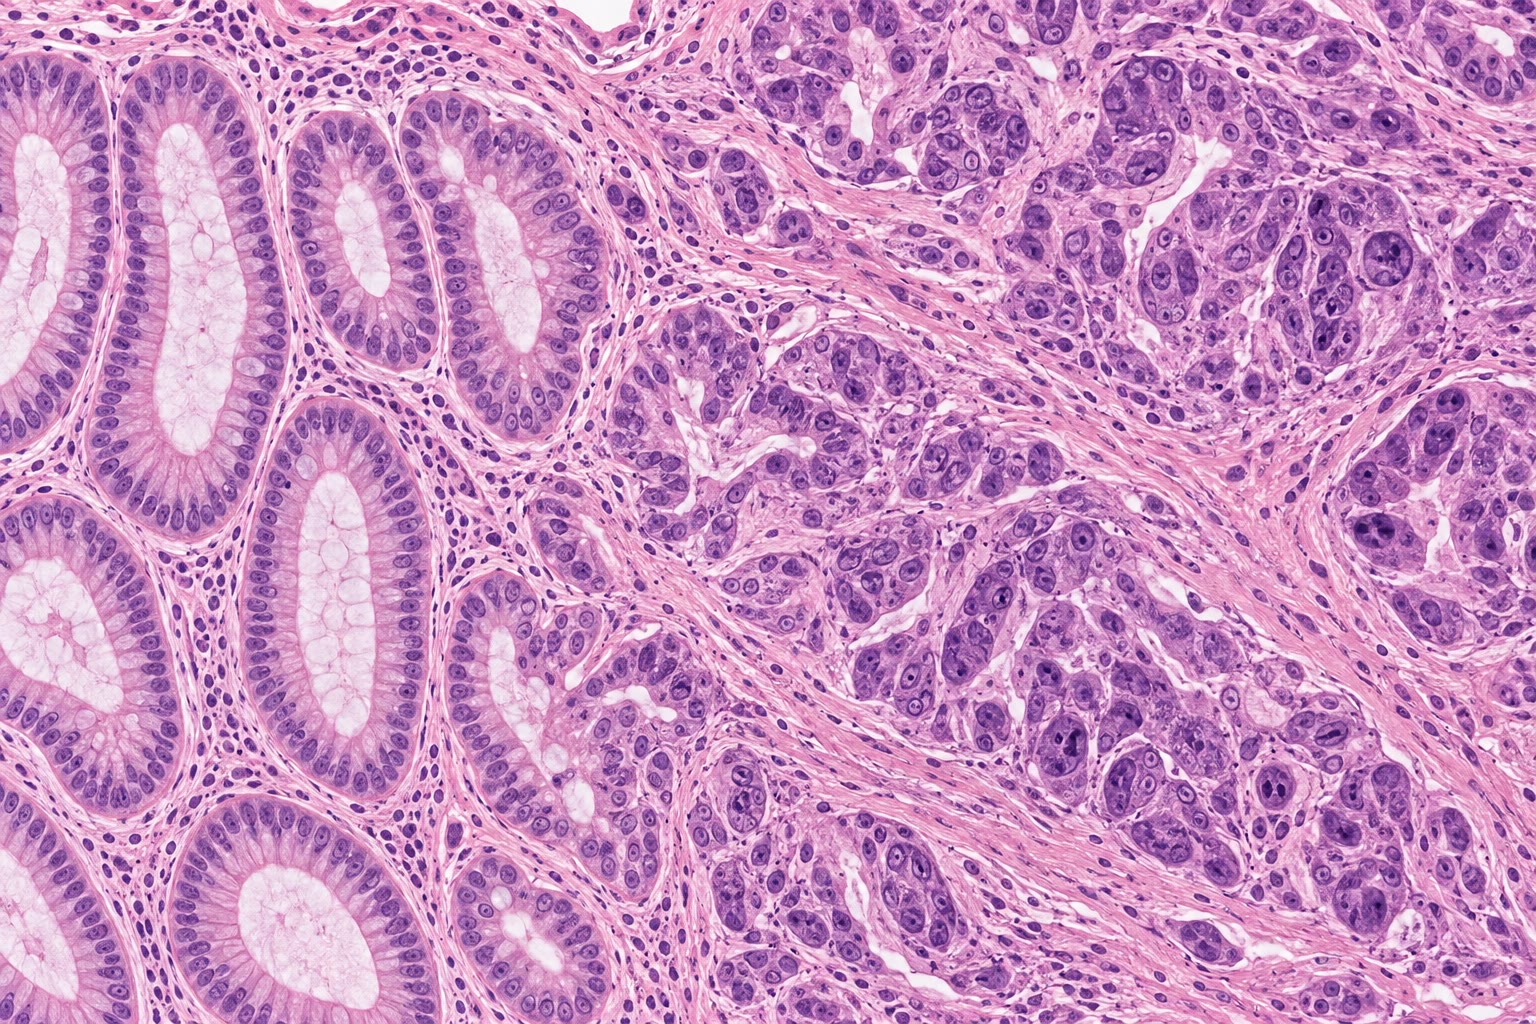
\includegraphics[width=0.56\linewidth]{images/book5/ai/b5-11-tumour-histology.jpg}

{\small كارسينوما عند حدها: على اليسار ظهارة غدية
منتظمة بأنوية منتظمة؛ وعلى اليمين خلايا متزاحمة بأنوية كبيرة
غير منتظمة تغزو السدى تحتها --- وهي الصورة التي يقرؤها
اختصاصي التشريح المرضي ليسمّي ورمًا خبيثًا.}
\end{omfigure}

\section{المورّثات التي تُصاب}

\begin{definition}[المورّثات الورمية والمورّثات الكابحة للورم]\label{def:b3:cancer-biology:genes}
\index{مورّثة ورمية}\index{مورّثة ورمية أولية}\index{مورّثة كابحة للورم}\index{Ras}\index{p53}\index{فرضية الإصابتين}
\emph{المورّثة الورمية الأولية} مورّثة سوية تعزز التكاثر أو
البقاء --- عامل نمو، أو مستقبله، أو بروتين إشارة، أو
عامل استنساخ، أو \omterm{def:b3:cell-cycle-apoptosis:cdk}{سيكلين} --- و\emph{المورّثة الورمية} صورة
طافرة منها تكون فعالة بلا إشارتها السوية: كطفرة نقطية
تحبس إنزيم \emph{Ras} الصغير من نمط GTPase في حالته المرتبطة بجزيء GTP (الغليسين~12 في
ربع السرطانات كلها)، أو تضخيم مورّثة المستقبل
HER2 أو مورّثة عامل الاستنساخ Myc، أو انتقال صبغي يلحم
\emph{BCR} بالكيناز \emph{ABL} في الابيضاض النقوي المزمن أو يضع
\emph{MYC} بجوار معزِّز جسم مضاد في لمفومة بيركيت. ويكفي أليل
طافر واحد: فالمورّثات الورمية تعمل عمل السائد. و\emph{المورّثة
الكابحة \omterm{def:b3:cancer-biology:hallmarks}{للورم}} تكبح التكاثر أو تفرض الموت أو الإصلاح
--- مثل Rb وp16 عند \omterm{def:b3:cell-cycle-apoptosis:checkpoints}{نقطة التقييد}، و\emph{p53} الحارس الذي
يوقف الخلية المتأذية أو يقتلها، وAPC في \omterm{prop:b3:cancer-biology:pathways}{مسلك Wnt} في القولون، و
PTEN، وBRCA1 وBRCA2، ومورّثات \omterm{prop:b3:dna-repair:fidelity}{إصلاح عدم التوافق} --- وعليها أن تفقد
أليليها معًا لتسهم: أي \emph{إصابتان}، الأولى موروثة غالبًا
في متلازمات \omterm{def:b3:cancer-biology:hallmarks}{السرطان} العائلية، والثانية جسدية. و\emph{p53}
مطفَّر في نصف سرطانات البشر ومسلكه معطَّل في معظم
الباقي.
\end{definition}

\begin{proof}[شواهد]
نقل روس (1911) ساركوما دجاج برشاحة خالية من الخلايا،
أي فيروس، ثم بيّن فارموس وبيشوب (1976) أن مورّثته المحوِّلة الوحيدة،
وهي \emph{src}، نسخة ملتقطة من مورّثة دجاج سوية
--- فالمورّثات الورمية مورّثات خلوية مبدَّلة. ونقل واينبرغ (1982)
DNA من كارسينوما مثانة بشرية إلى خلايا فأر مزروعة، فتحولت؛
وكانت القطعة المسؤولة \emph{RAS} بتغير قاعدة
واحدة، وكان التغير نفسه غائبًا عن نسيج المريض
السوي. وقارن كنودسون (1971) أطفالًا \omterm{def:b3:cancer-biology:hallmarks}{بورم} العين
الأرومي الشبكي: فمن لهم تاريخ عائلي أصيبوا بعدة أورام
في العينين معًا، باكرًا؛ ومن لا تاريخ لهم أصيبوا \omterm{def:b3:cancer-biology:hallmarks}{بورم} واحد، متأخرًا --- وهو ما يتسق
مع حاجة الحالات العائلية إلى حدث جسدي واحد، والمتفرقة إلى حدثين،
ومن ثم مع مورّثة يجب أن تُفقد نسختاها معًا. وقد استُنسخت \emph{RB}
عام 1986 وتبيّن أن كلا أليليها معطَّل في كل
\omterm{def:b3:cancer-biology:hallmarks}{ورم}.
\end{proof}

\begin{theorem}[الإصابات ومنحني العمر]\label{thm:b3:cancer-biology:armitage-doll}
\index{نموذج أرميتاج--دول}\index{التسرطن متعدد المراحل}
لنفترض أن سرطانًا يقتضي $k$ حدثًا مستقلًا محددًا للسرعة في سلالة
خلوية واحدة، يقع كل منها بمعدل ثابت $u$ في الخلية كل سنة،
في جمهرة من $N$ خلية قابلة، مع $ut \ll 1$. عندئذٍ يكون
احتمال أن تكون خلية معينة قد أصابتها الأحداث $k$ كلها عند العمر $t$
نحو $(ut)^{k}$، ويكون الخطر التراكمي في النسيج نحو $N(ut)^{k}$،
وتكون الحدوث --- أي الحالات الجديدة في السنة عند العمر $t$ ---
\[
I(t) \approx N\,k\,u^{k}\,t^{\,k-1},
\]
أي أسًّا للعمر بالأس $k - 1$: أي خطًا مستقيمًا ميله $k - 1$
على مخطط لوغاريتمي مزدوج. وعند من يرث أحد الأحداث،
يكون \omterm{def:b3:cancer-biology:hallmarks}{للسرطان} نفسه حدوث $\propto t^{\,k-2}$، أي أخفض بأسّ واحد.
\end{theorem}
\begin{proof}
كل حدث، بمعدل $u$، يكون قد وقع عند الزمن $t$ باحتمال
$1 - e^{-ut} \approx ut$؛ والأحداث مستقلة، فتكون قد وقعت كلها $k$
باحتمال $(ut)^{k}$، ولا يهم هنا الترتيب الذي
وقعت به. ومع $N$ خلية وأحداث نادرة، يكون
العدد المتوقع من الخلايا التي أتمت المتتالية
$N(ut)^{k}$، ويكون الحدوث مشتقه الزمني، أي $Nku^{k}t^{k-1}$.
ووراثةُ حدث واحد تترك $k - 1$ حدثًا لتقع: أي $(ut)^{k-1}$، والحدوث
$\propto t^{k-2}$. ولو كان ترتيب الأحداث مهمًا (فترتيب $1$ من $k!$
ترتيبًا هو الذي يقود إلى \omterm{def:b3:cancer-biology:hallmarks}{السرطان}) لتغير المعامل لا الأسّ.
\end{proof}

\begin{example}[قراءة الأسّ]\label{ex:b3:cancer-biology:exponent}
حدوث معظم الكارسينومات عند البالغين يرتفع بنحو الأسّ الخامس إلى
السادس من العمر --- من نحو $1$ في \num{100000} في السنة عند
الثلاثين إلى $1$ في $300$ عند الثمانين، أي بعامل $300$ مقابل عامل $2.7$
في العمر، و$2.7^{5.7} \approx 300$ --- وهو ما يوحي بستة أو سبعة
أحداث محددة للسرعة. والتقدير خام: فتوسع نسيلة
بعد كل إصابة يرفع عدد الخلايا المعرَّضة للتالية، فأحداث أقل
مع نمو نسيلي بينها تعطي الميل نفسه، وعدد
الطفرات \emph{القائدة} الموجودة في الأورام المسلسلة اثنتان إلى
ثماني. \omterm{def:b3:cancer-biology:hallmarks}{وورم} كنودسون الأرومي الشبكي يوافق عبارة المبرهنة الثانية
بالضبط: فالمرض المتفرق، وهو يحتاج إلى إصابتين، حدوثه
يرتفع مع العمر (خلال السنوات القليلة التي توجد فيها الأرومات الشبكية)؛ أما
المرض الوراثي، وهو يحتاج إلى واحدة، فحاضر بمعدل شبه ثابت
منذ الولادة ويضرب باكرًا ومرارًا.
\end{example}

\begin{omfigure}
\begin{tikzpicture}
\begin{axis}[
  width=0.68\linewidth, height=6cm,
  xmode=log, ymode=log,
  xmin=20, xmax=100, ymin=1e-6, ymax=1e-1,
  xlabel={العمر (بالسنوات)}, ylabel={الحدوث للشخص في السنة},
  xlabel style={font=\small, at={(axis description cs:0.5,-0.12)}, anchor=north},
  ylabel style={font=\small},
  tick label style={font=\small}, xtick={20,30,50,80}, xticklabels={20,30,50,80},
  clip=false,
]
\addplot[very thick, omThm, domain=20:100, samples=2] {1e-5*(x/30)^5.7};
\addplot[very thick, omDef, domain=20:100, samples=2] {3e-4*(x/30)^1};
\addplot[very thick, omMeth!70!black, domain=20:100, samples=2] {2e-3};
\node[font=\scriptsize, omThm, anchor=south west] at (axis cs:38,2.5e-6) {الكارسينومات: ميل $5$--$6$، أي ستة أو سبعة أحداث};
\node[font=\scriptsize, omDef, anchor=south west] at (axis cs:22,6e-4) {إصابتان: ميل 1};
\node[font=\scriptsize, omMeth!70!black, anchor=south west] at (axis cs:22,2.3e-3) {إصابة واحدة موروثة: ميل 0};
\end{axis}
\end{tikzpicture}

{\small الحدوث في مقابل العمر على محورين لوغاريتميين. \omterm{def:b3:cancer-biology:hallmarks}{فالسرطان} الذي يحتاج إلى $k$
حدثًا محددًا للسرعة يرتفع مثل $t^{k-1}$: وهو الخط الحاد لكارسينومات
البالغين، وحالتا كنودسون --- \omterm{def:b3:cancer-biology:hallmarks}{ورم} بإصابتين يرتفع
خطيًا، \omterm{def:b3:cancer-biology:hallmarks}{والورم} نفسه عند حامل إصابة موروثة واحدة، بمعدل
ثابت منذ الولادة.}
\end{omfigure}

\begin{proposition}[المسالك التي تُصاب]\label{prop:b3:cancer-biology:pathways}
\index{مسلك Ras--MAPK}\index{مسلك PI3K}\index{مسلك Wnt}
مئات مورّثات \omterm{def:b3:cancer-biology:hallmarks}{السرطان} تقع في عشرات المسالك، يعطّل \omterm{def:b3:cancer-biology:hallmarks}{الورم}
كلًا منها عند نقطة ما. فمسالك عامل النمو: مستقبل
كيناز التيروزين (EGFR، وHER2)، \omterm{def:b3:cancer-biology:genes}{وRas}، والشلال الكينازي Raf--MEK--ERK إلى
النواة، وبالتوازي PI3K--Akt--mTOR نحو البقاء والنمو،
يكبحه PTEN؛ \omterm{def:b3:cancer-biology:hallmarks}{والورم} ينشّط واحدًا منها، بأي مورّثة كانت.
ومكبح \omterm{def:b3:cell-cycle-apoptosis:cdk}{دورة الخلية}: \omterm{def:b3:cell-cycle-apoptosis:cdk}{السيكلين} D، وCdk4، وp16، وRb (\cref{ch:b3:cell-cycle-apoptosis}).
والحارس: \omterm{def:b3:cancer-biology:genes}{p53} ومنظماته. والموت: Bcl-2. وإشارات
التطور: Wnt (وAPC، و$\beta$-كاتينين) في القولون، وHedgehog في الجلد
والدماغ، وNotch في الخلايا التائية. وصيانة الجينوم: \omterm{prop:b3:dna-repair:fidelity}{إصلاح عدم التوافق}، و
\omterm{def:b3:dna-repair:dsb}{BRCA}، \omterm{def:b3:dna-repair:ddr}{وATM}. \omterm{def:b3:chromatin-epigenetics:nucleosome}{والصبغين}: كتبة \cref{ch:b3:chromatin-epigenetics}
ومعيدو تشكيله، وهم مطفَّرون في ثلث الأورام.
والخلود: مروّج \omterm{def:b3:cancer-biology:telomerase}{التيلوميراز}. ولأن المسلك سلسلة من
الخطوات، تكون الطفرات في مورّثات مختلفة بدائل --- \omterm{def:b3:cancer-biology:hallmarks}{فالورم} ذو
\omterm{def:b3:cancer-biology:genes}{Ras} الطافر نادرًا ما يحمل أيضًا EGFR طافرًا --- والأدوية ضد خطوة واحدة
قد تهزمها طفرة في خطوة لاحقة.
\end{proposition}

\begin{omfigure}
\begin{tikzpicture}[every node/.style={font=\scriptsize}, >=stealth]
  % membrane
  \draw[very thick, omDef] (0,3.6) -- (12,3.6); \draw[very thick, omDef] (0,3.3) -- (12,3.3);
  \node[above] at (1.0,3.65) {الخارج}; \node[below] at (1.0,3.25) {العصارة الخلوية};
  % receptor
  \draw[thick, fill=omProp!35] (3.7,3.0) rectangle (4.1,4.1); \draw[thick, fill=omProp!35] (4.3,3.0) rectangle (4.7,4.1);
  \node[above, align=center] at (4.2,4.15) {عامل نمو $\to$ مستقبل كيناز\\(EGFR، وHER2)}; \node[right, omThm, font=\tiny] at (4.75,4.0) {مضخَّم};
  % Ras
  \node[draw, thick, rounded corners, fill=omDef!20] (ras) at (4.2,2.3) {Ras--GTP};
  \node[right, omThm, font=\tiny] at (5.0,2.3) {G12: فعال دائمًا};
  \node[draw, thick, rounded corners, fill=omDef!20] (raf) at (4.2,1.4) {Raf $\to$ MEK $\to$ ERK};
  \node[right, omThm, font=\tiny] at (5.8,1.4) {BRAF V600E};
  \node[draw, thick, rounded corners, fill=omMeth!25] (myc) at (4.2,0.4) {Myc، والسيكلين D: التكاثر};
  \node[right, omThm, font=\tiny] at (6.4,0.4) {Myc مضخَّم};
  \draw[->, thick] (4.2,3.0) -- (ras); \draw[->, thick] (ras) -- (raf); \draw[->, thick] (raf) -- (myc);
  % PI3K branch
  \node[draw, thick, rounded corners, fill=omDef!20] (pi3k) at (9.6,2.3) {PI3K $\to$ Akt $\to$ mTOR};
  \node[draw, thick, rounded corners, fill=omMeth!25] (surv) at (9.6,0.4) {البقاء والنمو};
  \draw[->, thick] (4.7,3.0) .. controls (6.5,2.8) .. (pi3k.north west); \draw[->, thick] (pi3k) -- (surv);
  \node[draw, thick, rounded corners, fill=omThm!15] (pten) at (12.2,1.4) {PTEN}; \draw[-|, thick, omThm] (pten) -- (9.6,1.4);
  \node[below, omThm, font=\tiny] at (12.2,1.15) {محذوف};
  % p53 and Rb on the side
  \node[draw, thick, rounded corners, fill=omThm!15] (rb) at (1.2,0.4) {Rb، وp16}; \draw[-|, thick, omThm] (rb) -- (myc);
  \node[below, omThm, font=\tiny, align=center] at (1.2,0.15) {فُقد الأليلان};
  \node[draw, thick, rounded corners, fill=omThm!15] (p53) at (1.2,1.6) {p53}; \node[below, omThm, font=\tiny, align=center] at (1.2,1.35) {مطفَّر في نصف\\السرطانات};
  \draw[-|, thick, omThm] (p53) -- (1.2,0.65);
\end{tikzpicture}

{\small مسالك عامل النمو وأين تصيبها السرطانات. فالصناديق
الخضر هي النواتج، والزرق خطوات الإشارة التي تحبسها الطفرات
الورمية مفتوحةً، والحمر الكوابح التي تفقدها الأورام (والأشرطة تعلّم
التثبيط). ويحمل \omterm{def:b3:cancer-biology:hallmarks}{الورم} عادةً آفة منشّطة واحدة وآفة أو اثنتين
معطِّلة في هذا المخطط.}
\end{omfigure}

\section{الورم يتطور}

\begin{proposition}[التسرطن متعدد الخطوات]\label{prop:b3:cancer-biology:multistep}
\index{طفرة قائدة}\index{طفرة راكبة}\index{تطور نسيلي}\index{بصمة طفرية}
\omterm{def:b3:cancer-biology:hallmarks}{الورم} ناتج تطور جسدي: فالطفرة تولّد
متغايرات، والانتقاء داخل النسيج يحابي ما ينقسم
أكثر أو يموت أقل أو يفلت من قيد. والتسلسل القولوني المستقيمي
الذي حلّه فوغلشتاين هو النموذج: ففقد \emph{APC} ينتج
سليلة سليمة صغيرة؛ وطفرة \emph{KRAS} تتيح لها أن تنمو ورمًا
غديًا؛ وفقد \emph{SMAD4} أو \emph{TP53} يحوّله إلى كارسينوما؛
وتغيرات أخرى تتيح \omterm{def:b3:cancer-biology:metastasis}{الغزو}. وكل خطوة توسع نسيلي
يضاعف الخلايا المعرَّضة للخطوة التالية. \omterm{def:b3:cancer-biology:hallmarks}{والورم} المسلسل يحمل
آلاف الطفرات، منها حفنة --- اثنتان إلى ثماني عادةً
--- \emph{قائدة} منحت أفضلية انتقائية؛ والباقي
\emph{راكبة}، محمولة في النسيلة، وطيفها
سجل لما سببها: فالتحول C$\to$T عند بيريميدينين متجاورين من
الضوء فوق البنفسجي في الميلانوما، وG$\to$T من دخان التبغ في \omterm{def:b3:cancer-biology:hallmarks}{سرطان}
الرئة، وبصمات إنزيمات APOBEC، وبصمة \omterm{prop:b3:dna-repair:fidelity}{إصلاح عدم التوافق}
المعطوب، وبصمة الأفلاتوكسين --- وهي \emph{البصمات الطفرية}. والأورام
متغايرة، شجرة متفرعة من النسائل الفرعية، والنسيلة الفرعية التي
تقتل كثيرًا ما تكون أقلية عند التشخيص.
\end{proposition}

\begin{omfigure}
\begin{tikzpicture}[every node/.style={font=\scriptsize}, >=stealth]
  \foreach \x/\lab/\gene/\col/\r in {0/{ظهارة سوية}/{}/omDef!20/0.5, 2.6/{سليلة صغيرة}/{فقد APC (كلا الأليلين)}/omDef!35/0.7, 5.4/{ورم غدي}/{تنشيط KRAS}/omProp!40/1.0, 8.4/{كارسينوما}/{فقد SMAD4 أو TP53}/omThm!35/1.3, 11.6/{غازية، ونقيلية}/{قائدات أخرى،\\ولااستقرار}/omThm!60/1.5} {
    \draw[thick, fill=\col] (\x,0) circle (\r);
    \node[below, align=center] at (\x,-1.6) {\lab};
    \node[above, align=center, omThm] at (\x,1.6) {\gene};
  }
  \foreach \a/\b in {0.5/1.9, 3.3/4.4, 6.4/7.1, 9.7/10.1} \draw[->, very thick] (\a,0) -- (\b,0);
  \node[below] at (5.8,-2.3) {عشر إلى ثلاثين سنة؛ وكل خطوة توسع نسيلي يضاعف الخلايا المعرَّضة للخطوة التالية};
\end{tikzpicture}

{\small التسلسل القولوني المستقيمي. كل \omterm{prop:b3:cancer-biology:multistep}{طفرة قائدة} توسّع نسيلة،
وتوفر النسيلة الموسَّعة الخلايا التي يمكن أن تنشأ فيها القائدة
التالية؛ ويستغرق الطريق كله عقودًا، ولهذا يمنع تحرّي
السلائل السرطانَ.}
\end{omfigure}

\begin{method}[اختبار أيمز]\label{met:b3:cancer-biology:ames}
\index{اختبار أيمز}\index{مطفر}
لاختبار هل مادة كيميائية مطفِّرة، ومن ثم مسرطنة على الأرجح:
(1) خذ سلالة من \emph{Salmonella} فيها طفرة نقطية
في مورّثة اصطناع الهستيدين، فلا تستطيع النمو بلا هستيدين؛
(2) امزج المادة بمستخلص كبد، تحوّل إنزيماته كثيرًا من
المركبات إلى صورها المطفِّرة الفعالة، كما يفعل الجسم؛ (3)
ازرع نحو $10^{8}$ بكتيريا على أغار خالٍ من الهستيدين مع المزيج؛
(4) عُدّ المستعمرات التي تنمو --- فكل منها راجعة نشأت فيها طفرة
جديدة أعادت المورّثة؛ (5) قارن بالمعدل العفوي. فالزيادة
في الراجعات المتوقفة على الجرعة تعني أن المركب يسبب طفرات
نقطية. ومعظم المسرطنات المعروفة إيجابية؛ والاختبار رخيص،
ويستغرق يومين، والمركب الذي يخفق فيه يُفحص أكثر
قبل أن يُصنع.
\end{method}

\begin{definition}[الخلود واللااستقرار]\label{def:b3:cancer-biology:telomerase}
\index{تيلوميراز}\index{لااستقرار صبغي}\index{اختلال الصيغة!في السرطان}
الخلايا الجسدية السوية لا تيلوميراز فيها وتعدّ انقساماتها
بطول القسيم الطرفي (\cref{ch:b3:stem-cells}): فبعد نحو خمسين تشيخ،
والخلية التي تتخطى الشيخوخة بفقد \omterm{def:b3:cancer-biology:genes}{p53} وRb تمضي
حتى تُستنفد قسيماتها الطرفية وتلتحم صبغياتها وتنكسر
--- وهي أزمة تقتل معظم النسائل. والناجية النادرة قد أعادت تنشيط
\emph{التيلوميراز}، بطفرة في المروّج عادةً، وتكون خالدة؛
و\qty{90}{\%} من السرطانات تعبّر عن الإنزيم. وتترك الأزمة ندوبًا:
صبغيات ملتحمة ومكسورة، وتضخيمات، وحذوف، وانتقالات
--- وهو \emph{اللااستقرار الصبغي}، الذي يجعل، مع فقد نقطة تفتيش
المغزل وفقد استجابة \omterm{def:b3:cancer-biology:genes}{p53} لسوء الفرز، معظم الأورام
الصلبة مختلة الصيغة ويبقيها تولّد متغايرات. وأقلية من
الأورام لها بدلًا من ذلك نمط ظاهري مطفِّر من فقد \omterm{prop:b3:dna-repair:fidelity}{إصلاح عدم التوافق}،
بنمط صبغي سوي ومعدل طفرة نقطية أعلى ألف ضعف.
\end{definition}

\section{الورم نسيجًا}

\begin{proposition}[الأكسجين يحدد حجم ورم بلا أوعية]\label{prop:b3:cancer-biology:oxygen}
\index{تولد الأوعية}\index{حد الانتشار}\index{نقص الأكسجة}
لننظر في نسيج يستهلك الأكسجين بمعدل ثابت $q$ لوحدة الحجم،
يُمدّه الانتشار (بمعامل $D$) من وعاء يكون التركيز عند
جداره $c_{0}$. ففي بعد واحد عند الحالة المستقرة، $D\,
\mathrm{d}^{2}c/\mathrm{d}x^{2} = q$، ومنه $c(x) = c_{0} - qx^{2}/2D$ و
ينفد الأكسجين عند المسافة
\[
L = \sqrt{\frac{2Dc_{0}}{q}} .
\]
ومع $D = \qty{2e-9}{m^2/s}$ و$c_{0} = \qty{0.05}{mol/m^3}$ و$q =
\qty{0.03}{mol/m^3/s}$ (في \omterm{def:b3:cancer-biology:hallmarks}{ورم} يتنفس)، يكون $L \approx \qty{80}{\micro
m}$: فلا تستطيع خلية أن تعيش على أكثر من نحو مئة ميكرومتر من
شعيرة. والنسيلة التي لا أوعية لها تقف إذن عند
قطر ميليمتر أو اثنين، ولبها \omterm{def:b3:cell-cycle-apoptosis:apoptosis}{نخر} وحافتها
حية. ولتنمو أكثر يجب أن تحرّض \emph{\omterm{prop:b3:cancer-biology:oxygen}{تولد الأوعية}} --- فخلاياها
ناقصة الأكسجة تثبّت عامل الاستنساخ HIF، الذي يحرّض
VEGF، الذي يجعل الخلايا البطانية القريبة تبرعم نحوها. واقترح جوداه
فولكمان عام 1971 أن حجب هذه الخطوة يجوّع الأورام؛
والأجسام المضادة للعامل VEGF صارت اليوم معيارًا في عدة سرطانات، وإن كانت
الأورام تتكيف.
\end{proposition}
\begin{proof}
عند الحالة المستقرة يجب أن يتغير تدفق الانتشار $-D\,\mathrm{d}c/\mathrm{d}x$
مع $x$ بالسرعة نفسها التي يُستهلك بها الأكسجين: $\mathrm{d}(-D\,
\mathrm{d}c/\mathrm{d}x)/\mathrm{d}x = -q$، أي $D c'' = q$.
وبالتكامل مرتين مع $c(0) = c_{0}$ و$c'(L) = 0$ عند العمق
الذي لا يبقى عنده شيء (فلا تدفق بعده) نجد $c = c_{0} - qx^{2}/2D$
بعد استعمال $c(L) = 0$ لتثبيت $L$. والأرقام تتبع.
\end{proof}

\begin{omfigure}
\begin{tikzpicture}
\begin{axis}[
  width=0.6\linewidth, height=5.4cm,
  axis x line=bottom, axis y line=left,
  xmin=0, xmax=120, ymin=0, ymax=0.06,
  xlabel={المسافة من الشعيرة ($\unit{\micro m}$)}, ylabel={الأكسجين ($\unit{mol/m^3}$)},
  xlabel style={font=\small, at={(axis description cs:0.5,-0.12)}, anchor=north},
  ylabel style={font=\small},
  tick label style={font=\small}, xtick={0,40,80,120}, ytick={0,0.025,0.05},
  clip=false,
]
\addplot[very thick, omDef, domain=0:81.6, samples=40] {0.05 - 0.03*(x*1e-6)^2/(2*2e-9)};
\addplot[very thick, omDef, domain=81.6:120, samples=2] {0};
\fill[omThm!25] (axis cs:81.6,0) rectangle (axis cs:120,0.06);
\node[font=\scriptsize, omThm!70!black, anchor=south, align=center] at (axis cs:100,0.03) {لا أكسجين:\\نخر};
\node[font=\scriptsize, omDef, anchor=south west] at (axis cs:5,0.052) {$c(x) = c_{0} - qx^{2}/2D$};
\draw[dashed, gray] (axis cs:81.6,0) -- (axis cs:81.6,0.06); \node[font=\scriptsize, anchor=south west] at (axis cs:83,0.002) {$L$};
\end{axis}
\end{tikzpicture}

{\small الأكسجين في نسيج يتنفس يهبط قطعًا مكافئًا مع المسافة
عن أقرب شعيرة ويُستنفد عند $L = \sqrt{2Dc_{0}/q}$،
أي نحو \qty{80}{\micro m} هنا. \omterm{def:b3:cancer-biology:hallmarks}{والورم} بلا أوعية قشرة من
الخلايا الحية بذلك الثخن حول لبّ ميت.}
\end{omfigure}

\begin{omfigure}
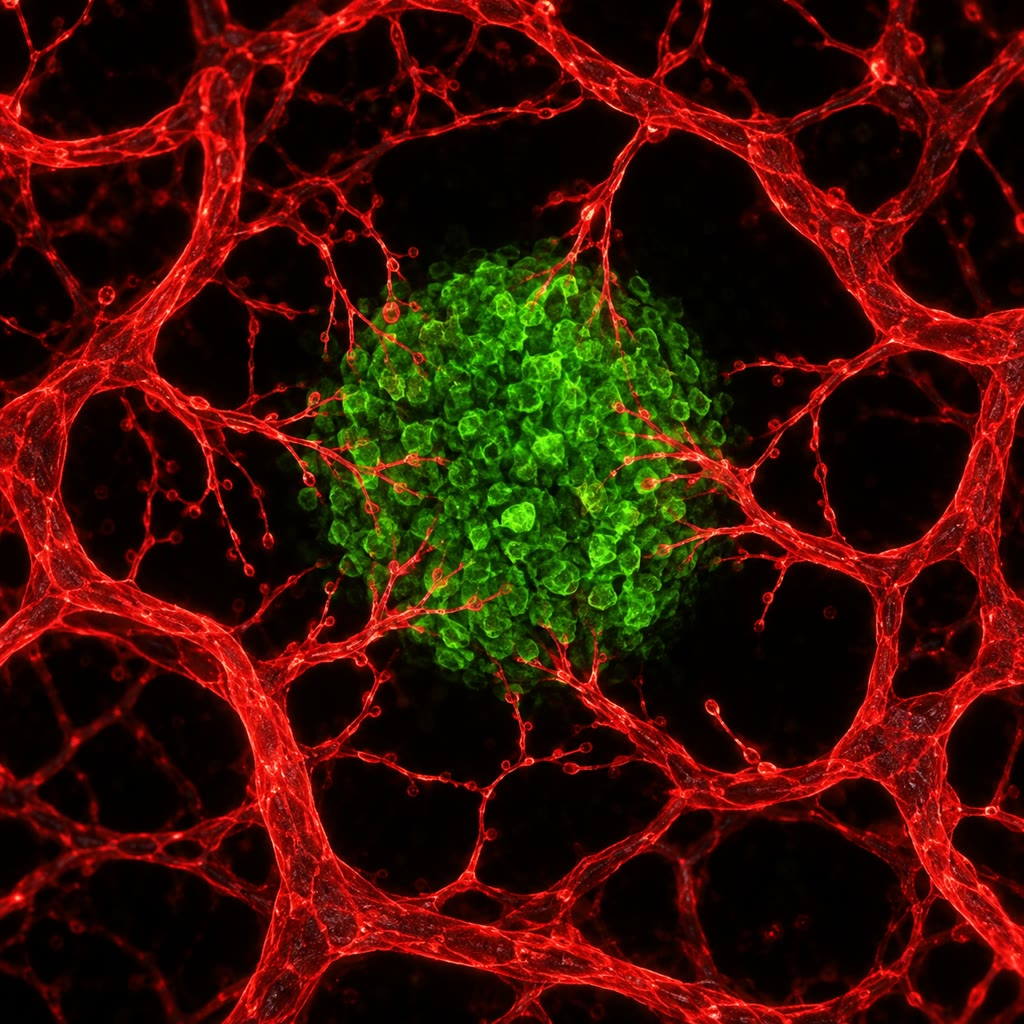
\includegraphics[width=0.36\linewidth]{images/book5/ai/b5-11-angiogenesis.jpg}\hspace{0.04\linewidth}
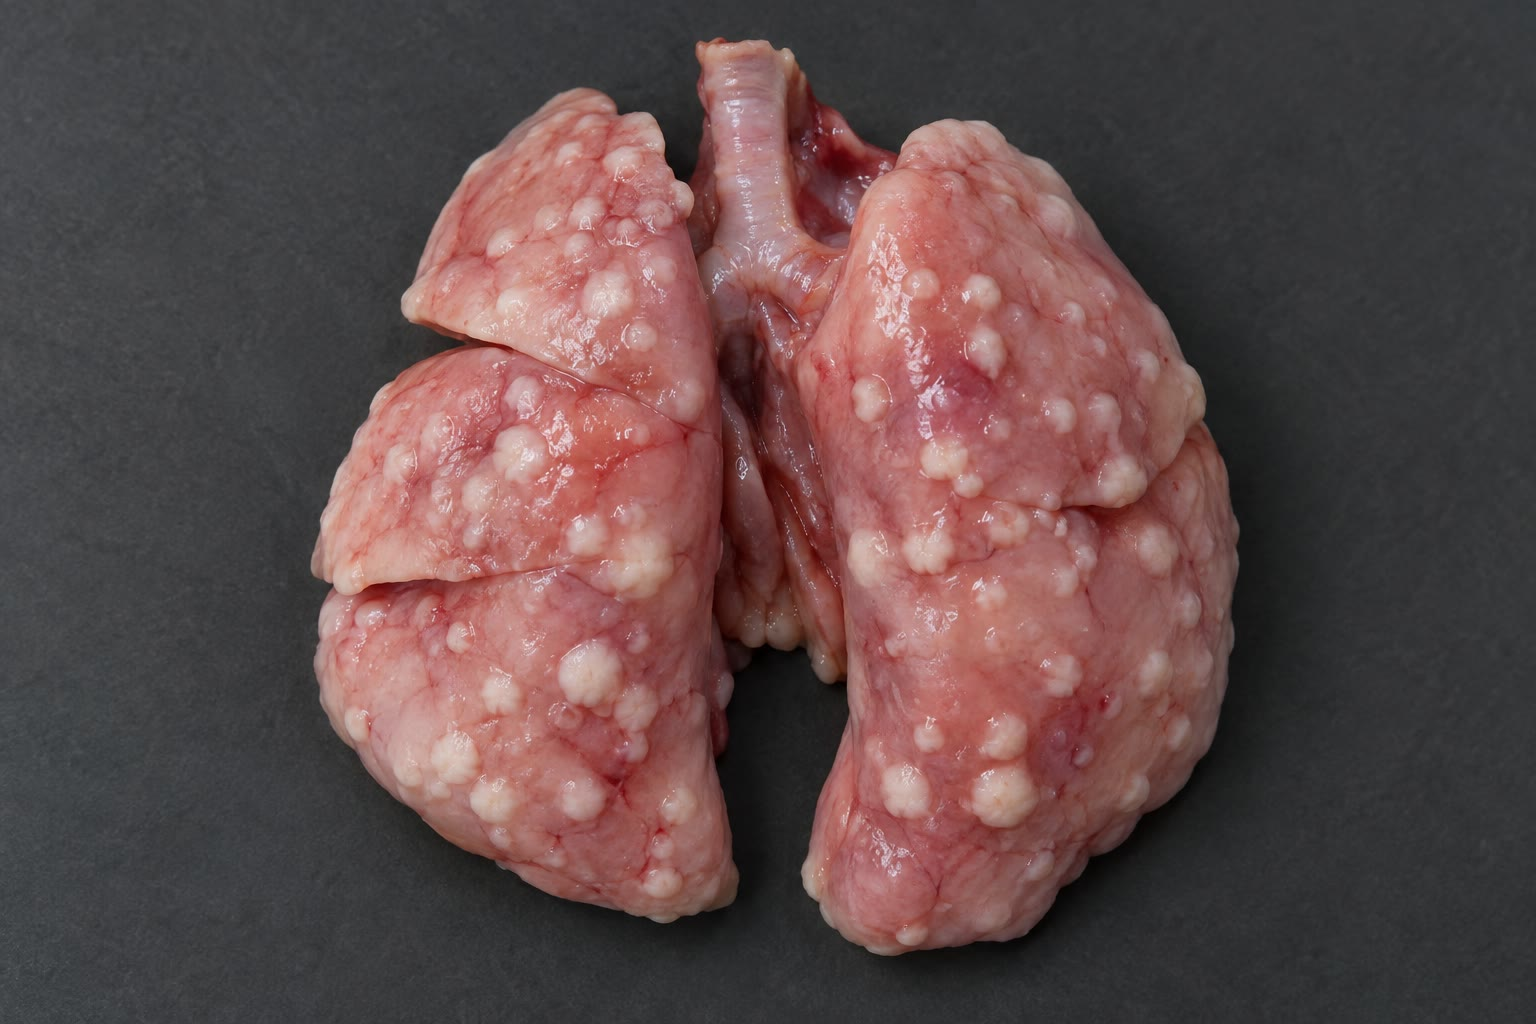
\includegraphics[width=0.54\linewidth]{images/book5/ai/b5-11-metastasis-lung.jpg}

{\small يسارًا: كروية ورمية (بالأخضر) تستقدم أوعية جديدة (بالأحمر)
من شبكة مجاورة --- أي تولد أوعية في مزرعة. يمينًا: رئة فأر
مرصّعة بالنقائل، أسّس كل مستعمرة منها خلية واحدة
نجت من رحلة الدم.}
\end{omfigure}

\begin{definition}[الغزو والنقيلة]\label{def:b3:cancer-biology:metastasis}
\index{غزو}\index{انتقال ظهاري--متوسطي}\index{البذرة والتربة}
لتنتقل خلية كارسينوما، يجب أن تغادر الظهارة --- فتفقد
وصلاتها الخلوية وقطبيتها وتكتسب حركية، وهو
\emph{انتقال ظهاري--متوسطي} تقوده عوامل استنساخ
تُستعمل عادةً في التطور الجنيني --- وأن تحلّل الغشاء
القاعدي والحشوة ببروتيازات مفرَزة، وأن تعبر جدار وعاء دموي
أو لمفي، وأن تنجو في الدوران (فأقل من واحدة في عشرة
آلاف تنجو، إذ يقتلها القص، وغياب الالتصاق، و
الخلايا القاتلة الطبيعية)، وأن تستقر في سرير شعري في عضو آخر، وأن تعبر
خارجه، وأن تنمو هناك. وأين تنمو ليس عشوائيًا: \omterm{def:b3:cancer-biology:hallmarks}{فسرطان} الثدي يذهب إلى
العظم والرئة والكبد والدماغ، \omterm{def:b3:cancer-biology:hallmarks}{وسرطان} القولون إلى الكبد، \omterm{def:b3:cancer-biology:hallmarks}{وسرطان} البروستاتة
إلى العظم --- وهي \emph{بذرة وتربة} باجيت عام 1889، ويفسرها جزئيًا
جريان الدم وجزئيًا التلاؤم بين الخلية وإشارات
النسيج. وقد ترقد الخلية المنتشرة سنين قبل أن تنمو،
ولهذا تنتكس السرطانات بعد عقد من شفاء ظاهر. \omterm{def:b3:cancer-biology:hallmarks}{والنقيلة}
تسبب تسع وفيات من عشر من الأورام الصلبة، وهي الخطوة الأقل
فهمًا.
\end{definition}

\begin{proposition}[الإفلات من الجهاز المناعي]\label{prop:b3:cancer-biology:immune}
\index{إفلات مناعي}\index{مثبط نقاط التفتيش}\index{مستضد جديد}
طفرات \omterm{def:b3:cancer-biology:hallmarks}{الورم} تخلق \emph{مستضدات جديدة}، وهي ببتيدات لا تعرضها
خلية سوية، وتتعرفها الخلايا التائية السامة وتقتل خلايا \omterm{def:b3:cancer-biology:hallmarks}{الورم} --- وهو
سبب كثرة السرطانات عند المرضى المثبَّطين مناعيًا وسبب
استجابة الأورام كثيرة الطفرات (الميلانوما، والرئة، والقولون المعوز
\omterm{prop:b3:dna-repair:fidelity}{إصلاح عدم التوافق}) للمعالجة المناعية أحسن استجابة. \omterm{def:b3:cancer-biology:hallmarks}{والورم} البيّن
سريريًا هو الذي أفلت: بفقد جزيئات MHC التي تعرض
الببتيدات، وبإفراز عوامل كابتة، وباستقدام خلايا تائية
منظِّمة، وقبل ذلك كله بالتعبير عن PD-L1، الذي يشتبك مع
المستقبل المثبط PD-1 على الخلايا التائية فيطفئها، وهو المكبح
نفسه الذي ينهي الاستجابة المناعية عادةً
(\cref{ch:b3:adaptive-immunity}). والأجسام المضادة التي تحجب PD-1 أو PD-L1،
أو المكبح الأسبق CTLA-4، تطلق الخلايا التائية؛ وفي نسبة من
المرضى --- خمس إلى نصف بحسب \omterm{def:b3:cancer-biology:hallmarks}{الورم} --- تحدث
هدأة دائمة لسرطانات لم تكن تُعالج، وتكون آثارها
الجانبية مناعةً ذاتية، وهي الوظيفة الأخرى للمكبح.
\end{proposition}

\section{الأسباب والعلاجات}

\begin{proposition}[الأسباب]\label{prop:b3:cancer-biology:causes}
\index{مسرطن}\index{فيروس مسرطن}
يسبب السرطانَ كل ما يرفع معدل الأحداث في
المبرهنة أو عدد الخلايا المعرَّضة. ومنها \emph{المسرطنات الكيميائية}،
ومعظمها مطفِّر بعد تفعيله في الكبد: كالسبعين
مسرطنًا في دخان التبغ، التي تسبب ثلث وفيات \omterm{def:b3:cancer-biology:hallmarks}{السرطان} و
ترفع خطر \omterm{def:b3:cancer-biology:hallmarks}{سرطان} الرئة خمسة عشر إلى خمسة وعشرين ضعفًا؛ والأفلاتوكسين
من الحبوب المعفّنة؛ والأسبستوس، وهو ليس مطفِّرًا بل مهيّجًا
مزمنًا. و\emph{الإشعاع}: الضوء فوق البنفسجي للجلد (وهي ثنائيات
\cref{ch:b3:dna-repair})، والإشعاع المؤيّن للابيضاض والدرق
والثدي. و\emph{الأخماج}، وهي سدس السرطانات عالميًا: كفيروسات
\omterm{def:b3:cancer-biology:hallmarks}{الورم} الحليمي، التي يهدم بروتيناها E6 وE7 بروتين \omterm{def:b3:cancer-biology:genes}{p53} ويعطّلان
Rb ويسببان كل سرطانات عنق الرحم تقريبًا (وثمة لقاح يمنعها اليوم)؛
وفيروسا التهاب الكبد B وC في \omterm{def:b3:cancer-biology:hallmarks}{سرطان} الكبد؛ وفيروس إبشتاين--بار في
اللمفومات؛ و\emph{Helicobacter pylori} في \omterm{def:b3:cancer-biology:hallmarks}{سرطان} المعدة، عبر عقود
من الالتهاب. و\emph{الطفرات الموروثة} في \omterm{def:b3:cancer-biology:genes}{مورّثة كابحة للورم}، وهي
الإصابة الأولى منذ الولادة، في نحو \qty{5}{\%} من السرطانات. والمصادفة: فمعظم
الطفرات في \omterm{def:b3:cancer-biology:hallmarks}{ورم} نشأت من أخطاء التضاعف العادية،
فالأنسجة الأكثر انقسامًا --- القولون، والجلد، والدم ---
فيها أكثر السرطانات، ويرتفع الخطر مع العمر مهما فعل المرء.
\end{proposition}

\begin{theorem}[لماذا يخفق دواء واحد وقد لا يخفق اثنان]\label{thm:b3:cancer-biology:goldie-coldman}
\index{نموذج غولدي--كولدمان}\index{مقاومة الأدوية}\index{المعالجة التوليفية}
ليكن \omterm{def:b3:cancer-biology:hallmarks}{ورم} من $N$ خلية قد نتج عن انقسامات متعاقبة
من خلية واحدة، ولتنشأ طفرة تمنح مقاومة لدواء معين
بمعدل $\mu$ لكل انقسام خلية. عندئذٍ يكون احتمال ألا يحوي
\omterm{def:b3:cancer-biology:hallmarks}{الورم} \emph{أي} خلية مقاومة حين يبدأ العلاج نحو
\[
P_{0} \approx e^{-\mu N},
\]
فمن أجل $\mu N \gg 1$ تكون المقاومة موجودة سلفًا بيقين شبه تام.
ومن أجل دوائين بآليتي مقاومة مستقلتين، تنشأ خلية مقاومة
لكليهما بمعدل نحو $\mu_{1}\mu_{2}$ لكل انقسام، ويكون $P_{0}
\approx e^{-\mu_{1}\mu_{2}N}$: فمع $N = 10^{9}$ و$\mu = 10^{-7}$،
يواجه دواء واحد $\mu N = 100$ نسيلة مقاومة وسطيًا، ويواجه دواءان
احتمالًا قدره $10^{-5}$ لوجود خلية واحدة مقاومة للاثنين.
\end{theorem}
\begin{proof}[برهان جزئي]
النمو من $1$ إلى $N$ خلية يستغرق نحو $N$ انقسامًا جملةً (فالشجرة
ذات $N$ ورقة فيها $N - 1$ عقدة داخلية). فإذا أُنتجت خلية مقاومة
عند كل انقسام باحتمال $\mu$، وإذا كانت ذريتها، بالتقريب
الأول، لا تموت ولا تفوق البقية نموًا، كان
عدد أحداث المقاومة بواسونيًا بمتوسط $\mu N$، وكان
احتمال ألا يقع أي منها $e^{-\mu N}$. والآليات المستقلة تضرب
احتمالات كل انقسام. والتقريب يهمل أن الطافرات الباكرة
تترك نسائل مقاومة أكبر --- والتوزيع الكامل هو توزيع
لوريا ودلبروك المتناوَل في كتاب السنة~الثانية --- لكن
احتمال ألا يوجد \emph{أي} طافر، وهو ما يقرر هل يمكن شفاء
\omterm{def:b3:cancer-biology:hallmarks}{الورم}، هو بالضبط حد بواسون.
\end{proof}

\begin{example}[العلاجات ومنطقها]\label{ex:b3:cancer-biology:therapy}
الجراحة والمعالجة الشعاعية تزيلان ورمًا موضعيًا أو تقتلانه؛ والإشعاع
يقتل بالكسور المزدوجة الطاق، وتجزئته إلى جرعات يومية
تتيح للنسيج السوي أن يصلح بينها (\cref{ch:b3:dna-repair}).
أما المعالجة الكيميائية السامة للخلايا --- العوامل المؤلكلة، ومضادات المستقلَبات،
وسموم الأنيبيبات الدقيقة، ومثبطات التوبوإيزوميراز --- فتقتل الخلايا المنقسمة
من أي نوع، وخلايا \omterm{def:b3:cancer-biology:hallmarks}{الورم} أكثر قليلًا، وتتبع
قانون \emph{القتل اللوغاريتمي}: إذ يقتل كل شوط نسبة ثابتة، ولتكن
\qty{99}{\%}، فتخفض ستة أشواط $10^{12}$ خلية إلى واحدة، و
تلزم الأشواط الستة نفسها سواء كان \omterm{def:b3:cancer-biology:hallmarks}{الورم} كبيرًا أم صغيرًا؛
وشعر المريض وأمعاؤه ونقيه، وهي تنقسم أيضًا، تحدد الجرعة.
والمعالجة الموجَّهة تهاجم آفة يعتمد عليها \omterm{def:b3:cancer-biology:hallmarks}{الورم}: فالإيماتينيب
يحجب كيناز BCR--ABL وحوّل الابيضاض النقوي المزمن من
مرض قاتل إلى مرض مزمن؛ والتراستوزوماب يربط HER2؛ ومثبطات
PARP، ومثبطات Cdk4/6، والفينيتوكلاكس في الفصول السابقة
يستثمر كل منها عيبًا واحدًا. والمعالجة المناعية تطلق الخلايا التائية. و
المبرهنة تقول كيف ينبغي أن تُستعمل: في توليفة، وباكرًا، حين يكون $N$
أصغر ما يكون --- وهو ما تفعله المعالجة الكيميائية المساعدة بعد الجراحة
--- وبأدوية لا تتداخل آليات مقاومتها. و
\omterm{def:b3:cancer-biology:hallmarks}{الورم} جمهرة تتطور، والعلاج انتقاء.
\end{example}

\begin{omfigure}
\begin{tikzpicture}
\begin{axis}[
  width=0.7\linewidth, height=5.6cm,
  axis x line=bottom, axis y line=left,
  xmin=0, xmax=8, ymin=1, ymax=1e13, ymode=log,
  xlabel={أشواط المعالجة الكيميائية}, ylabel={خلايا الورم},
  xlabel style={font=\small, at={(axis description cs:0.5,-0.12)}, anchor=north},
  ylabel style={font=\small},
  tick label style={font=\small}, xtick={0,2,4,6,8},
  clip=false,
]
\addplot[very thick, omDef, mark=*, mark size=1.2pt] coordinates {(0,1e12) (1,1e10) (2,1e8) (3,1e6) (4,1e4) (5,1e2) (6,1)};
\addplot[very thick, omThm, mark=*, mark size=1.2pt] coordinates {(0,1e12) (1,1.01e10) (2,1.02e8) (3,1.04e6) (4,1.1e4) (5,200) (6,300) (7,600) (8,1200)};
\addplot[dashed, gray, domain=0:8, samples=2] {1e9};
\node[font=\scriptsize, gray, anchor=south west] at (axis cs:0.2,1.3e9) {قابل للكشف، $10^{9}$};
\node[font=\scriptsize, omDef, anchor=south west] at (axis cs:0.3,1e4) {قتل \qty{99}{\%} في الشوط};
\node[font=\scriptsize, omThm, anchor=south west] at (axis cs:5.2,3e3) {خلية مقاومة واحدة في البداية: انتكاس};
\end{axis}
\end{tikzpicture}

{\small قانون القتل اللوغاريتمي. يقتل كل شوط النسبة نفسها من الخلايا،
فيتقلص \omterm{def:b3:cancer-biology:hallmarks}{الورم} بعدد ثابت من العقود في الشوط ويصير
غير قابل للكشف قبل زواله بكثير (بالأزرق)؛ أما خلية مقاومة
واحدة موجودة سلفًا فتنجو من كل شوط وتعيد النمو (بالأحمر).}
\end{omfigure}

\begin{remark}[ما الذي تغيّر]\label{rem:b3:cancer-biology:changed}
نصف من يُشخَّص \omterm{def:b3:cancer-biology:hallmarks}{بالسرطان} في بلد غني ينجو اليوم
عشر سنوات، مقابل الربع عام 1970. وجاء المكسب من
الوقاية (التبغ، ولقاحا التهاب الكبد وفيروس \omterm{def:b3:cancer-biology:hallmarks}{الورم} الحليمي، والتحري
عن السلائل وآفات عنق الرحم)، ومن الكشف الأبكر، ومن
العلاجات التي تتبع من بيولوجيا هذا الفصل ---
المعالجة الكيميائية التوليفية التي تشفي معظم ابيضاضات الأطفال
وسرطانات الخصية، والأدوية الموجَّهة، والمعالجات المناعية. أما ما
لم يتغير فالمرض النقيلي، الذي تفسره البيولوجيا لكنها
لا تشفيه بعد؛ وستأتي المكاسب التالية من معاملة \omterm{def:b3:cancer-biology:hallmarks}{الورم} بوصفه
ما هو عليه، أي جمهرة تتطور تحت الانتقاء الذي يفرضه العلاج.
\end{remark}

\section{تمارين}

\begin{exercise}[$\star$]\label{exo:b3:cancer-biology:1}
ميّز \omterm{def:b3:cancer-biology:genes}{المورّثة الورمية} من \omterm{def:b3:cancer-biology:genes}{المورّثة الكابحة للورم} في الآلية،
وفي عدد الأليلات التي يجب أن تتغير، وبمثالين لكل منهما.
\end{exercise}

\begin{exercise}[$\star$]\label{exo:b3:cancer-biology:2}
عدّد \omterm{def:b3:cancer-biology:hallmarks}{سمات السرطان}، وسمِّ لكل منها مورّثة من هذا الفصل أو من
فصل سابق يوفرها تبدلها.
\end{exercise}

\begin{exercise}[$\star$]\label{exo:b3:cancer-biology:3}
ماذا لاحظ كنودسون في \omterm{def:b3:cancer-biology:hallmarks}{الورم} الأرومي الشبكي الوراثي والمتفرق،
وما الذي استنتجه؟
\end{exercise}

\begin{exercise}[$\star$]\label{exo:b3:cancer-biology:4}
فسّر \omterm{met:b3:cancer-biology:ames}{اختبار أيمز} ولماذا يُضاف مستخلص كبد.
\end{exercise}

\begin{exercise}[$\star\star$]\label{exo:b3:cancer-biology:5}
حدوث \omterm{def:b3:cancer-biology:hallmarks}{سرطان} $2\times 10^{-5}$ في السنة عند العمر $40$
و$2\times 10^{-3}$ عند العمر $80$. قدّر أسّ
قانون الأسّ العمري وعدد الأحداث المحددة للسرعة الذي يوحي به.
\end{exercise}

\begin{exercise}[$\star\star$]\label{exo:b3:cancer-biology:6}
باستعمال \cref{prop:b3:cancer-biology:oxygen} مع $D =
\qty{2e-9}{m^2/s}$ و$c_{0} = \qty{0.05}{mol/m^3}$، احسب $L$ في
نسيج يستهلك \qty{0.01}{mol/m^3/s} وفي \omterm{def:b3:cancer-biology:hallmarks}{ورم} يستهلك ثلاثة
أضعاف ذلك. ولماذا يصير \omterm{def:b3:cancer-biology:hallmarks}{الورم} السريع النمو نخرًا أبكر؟
\end{exercise}

\begin{exercise}[$\star\star$]\label{exo:b3:cancer-biology:7}
\omterm{def:b3:cancer-biology:hallmarks}{ورم} من $10^{11}$ خلية يُعالج بدواء يقتل
\qty{99.9}{\%} في الشوط. فكم شوطًا يلزم لخفضه دون خلية
واحدة؟ ولماذا يكون \omterm{def:b3:cancer-biology:hallmarks}{الورم} غير قابل للكشف بعد شوطين مع أن
$10^{5}$ خلية تبقى، وماذا يعني ذلك لإيقاف العلاج؟
\end{exercise}

\begin{exercise}[$\star\star$]\label{exo:b3:cancer-biology:8}
فسّر لماذا نادرًا ما تُوجد طفرة في EGFR وطفرة في KRAS
في \omterm{def:b3:cancer-biology:hallmarks}{ورم} الرئة نفسه، ولماذا كثيرًا ما ينتكس \omterm{def:b3:cancer-biology:hallmarks}{ورم} عولج بمثبط
EGFR بطفرة في KRAS.
\end{exercise}

\begin{exercise}[$\star\star$]\label{exo:b3:cancer-biology:9}
بروتينا فيروس \omterm{def:b3:cancer-biology:hallmarks}{الورم} الحليمي E6 وE7 يعطلان \omterm{def:b3:cancer-biology:genes}{p53} وRb. فسّر
كيف يقود ذلك \omterm{def:b3:cancer-biology:hallmarks}{سرطان} عنق الرحم، ولماذا يستغرق عقودًا، ولماذا
يمنعه لقاح يُعطى قبل النشاط الجنسي.
\end{exercise}

\begin{exercise}[$\star\star\star$]\label{exo:b3:cancer-biology:10}
وسّع حجة أرميتاج--دول لتسمح لكل إصابة بأن توسّع
نسيلتها بعامل $g$ قبل التالية: بيّن أن للحدوث الأسّ
نفسه للزمن $t$ لكن بمعامل مضروب في $g^{k-1}$، وناقش
لماذا يكون $k$ المطابق من منحني عمر حدًا أعلى لعدد
المورّثات القائدة.
\end{exercise}

\begin{exercise}[$\star\star\star$]\label{exo:b3:cancer-biology:11}
باستعمال \cref{thm:b3:cancer-biology:goldie-coldman}، قارن بين (أ) معالجة
\omterm{def:b3:cancer-biology:hallmarks}{ورم} من $10^{9}$ خلية بالدواء A ستة أشواط ثم بالدواء B ستة،
و(ب) إعطاء A وB معًا من البداية، حين يكون $\mu_{A} =
\mu_{B} = 10^{-7}$. احسب $P_{0}$ لكل استراتيجية وفسّر لماذا
تكون التوليفة الباكرة هي القاعدة.
\end{exercise}

\begin{exercise}[$\star\star\star$]\label{exo:b3:cancer-biology:12}
مفارقة بيتو: للفيل مئة ضعف خلايا
الإنسان ويعيش عمرًا مماثلًا، ومع ذلك لا \omterm{def:b3:cancer-biology:hallmarks}{سرطان} عنده أكثر. باستعمال مبرهنة
هذا الفصل، قل ما التوقع الساذج، واقترح آليتين
يمكن أن تكون الحيوانات الكبيرة قد حلت بهما المسألة (فللفيل
عشرون نسخة من \emph{TP53}).
\end{exercise}

\section{مسألة: حساب ورم}

\begin{problem}[{مسألة نهاية الأسبوع --- ورم نامٍ من خلية واحدة و
موقوت حتى الكشف، ومنحني عمره مقروءًا لعدد الإصابات، و
إمداده بالأكسجين ولبه النخر محسوبين، وعلاجه مخططًا
في مواجهة يقين المقاومة، وتنتهي إلى السنوات حتى الكشف،
وعمق الورم الحي حول وعاء واحتمال أن تشفي
التوليفة}]
\label{pb:b3:cancer-biology:1}
معطيات: حجم خلية \omterm{def:b3:cancer-biology:hallmarks}{الورم} \qty{1000}{\micro m^3}؛ وزمن المضاعفة
\qty{100}{d}؛ والكشف عند \qty{1}{cm^3}؛ والحمل المميت \qty{1}{kg}.
ومنحني العمر: الحدوث $1\times 10^{-5}$ في السنة عند $30$ و$3\times
10^{-3}$ عند $80$. والأكسجين: $D = \qty{2e-9}{m^2/s}$، و$c_{0} =
\qty{0.05}{mol/m^3}$، و$q = \qty{0.03}{mol/m^3/s}$ في \omterm{def:b3:cancer-biology:hallmarks}{الورم}؛ والشعيرات
في \omterm{def:b3:cancer-biology:hallmarks}{ورم} متوعٍّ تبعد \qty{150}{\micro m} بعضها عن بعض. والعلاج: كل
شوط يقتل \qty{99}{\%}؛ ومعدل طفرة المقاومة $10^{-7}$ لكل
انقسام لكل دواء؛ وشوط كل ثلاثة أسابيع؛ ويعيد \omterm{def:b3:cancer-biology:hallmarks}{الورم} النمو
بين الأشواط بزمن المضاعفة نفسه.

\medskip
\noindent\textbf{الجزء الأول --- النمو.}
\begin{enumerate}
  \item كم خلية في \qty{1}{cm^3}؟ وكم مضاعفةً من خلية
        واحدة؟
  \item كم سنة من الخلية المؤسِّسة إلى الكشف؟
  \item كم مضاعفةً، وكم سنة، من الكشف إلى الحمل
        المميت؟ قارن الفترتين.
  \item كثير من الأورام يُكشف عند \qty{1}{cm^3} لكنها كانت تنمو
        خمس سنوات فقط. فما الذي يجب أن يكون قد صحّ عن زمن المضاعفة
        في البداية، أو عن قانون النمو؟
  \item لا تنقسم إلا نسبة $f$ من خلايا \omterm{def:b3:cancer-biology:hallmarks}{الورم} في أي
        وقت (وهي نسبة النمو)، وتموت نسبة منها. فإذا دارت الخلايا
        في \qty{2}{d} لكن \omterm{def:b3:cancer-biology:hallmarks}{الورم} يتضاعف في $100$، فماذا يقول
        ذلك عن توازن الولادة والموت؟
  \item لماذا تعفي المعالجة الكيميائية ذات القتل اللوغاريتمي نفسها ورمًا بطيء
        النمو أكثر مما تعفي سريعه، ومع ذلك يعيد السريع
        النمو أسرع بين الأشواط؟
\end{enumerate}

\medskip
\noindent\textbf{الجزء الثاني --- الإصابات.}
\begin{enumerate}[resume]
  \item من الحدوثين، احسب الأسّ $k - 1$ في
        منحني العمر وعدد الأحداث $k$ الذي يقتضيه.
  \item إذا وقع كل حدث بمعدل $u = 10^{-6}$ في الخلية كل سنة في
        $N = 10^{8}$ خلية قابلة، فبماذا تتنبأ المبرهنة
        للخطر التراكمي عند العمر $70$ بقيمة $k$ التي حسبتها؟ أهو
        معقول؟ وما الذي ينقص؟
  \item أعد ذلك مع توسع نسيلي بعامل $g = 100$ بعد كل
        من الإصابات $k - 1$ الأولى، مستعملًا
        \cref{exo:b3:cancer-biology:10}.
  \item حاملة ترث إصابة واحدة. فبأي عامل يرتفع حدوثها عند
        العمر $40$، إذا لم تتغير المعدلات الأخرى؟ (قارن
        $(ut)^{k-1}$ بالمقدار $(ut)^{k}$ عند $t = 40$.)
  \item التدخين يضرب $u$ لأحد الأحداث في $10$. فبأي
        عامل يرتفع الحدوث إذا كان ذلك الحدث واحدًا من $k$؛
        وإذا كان اثنين منها؟
  \item فسّر لماذا يخفض الإقلاع عن التدخين عند الخمسين خطر \omterm{def:b3:cancer-biology:hallmarks}{سرطان}
        الرئة دون خطر المدخن المستمر، لكنه لا يبلغ به قط خطر
        من لم يدخن قط.
\end{enumerate}

\medskip
\noindent\textbf{الجزء الثالث --- الإمداد.}
\begin{enumerate}[resume]
  \item احسب عمق نفاذ الأكسجين $L$ في \omterm{def:b3:cancer-biology:hallmarks}{الورم}.
  \item كروية بلا أوعية: ما أقصى قطر تكون عنده كل
        خلية مؤكسجة؟ وما ثخن الحافة الحية
        في كروية قطرها \qty{2}{mm}، وما نسبة حجمها
        الحية؟
  \item في \omterm{def:b3:cancer-biology:hallmarks}{ورم} متوعٍّ شعيراته تبعد \qty{150}{\micro m}
        بعضها عن بعض، أتكون كل خلية مؤكسجة؟ وأي الخلايا ناقصة الأكسجة، و
        لماذا يهم ذلك في المعالجة الشعاعية (فالأكسجين يثبّت أذية الإشعاع)
        وفي انتقاء الخلايا الطافرة في \omterm{def:b3:cancer-biology:genes}{p53}؟
  \item دواء ينصّف كثافة شعيرات \omterm{def:b3:cancer-biology:hallmarks}{الورم}. أعد حساب
        المباعدة وقل ماذا يحدث للخلايا في منتصف المسافة بين
        الأوعية.
  \item الخلايا ناقصة الأكسجة تتحول إلى التحلل السكري، فتصنع \qty{2}{ATP} لكل
        غلوكوز بدل $30$. فبأي عامل يجب أن ترفع التقاط
        الغلوكوز لتحفظ إمدادها من ATP، وكيف يُستثمر ذلك في
        تصوير الأورام؟
  \item فسّر لماذا نادرًا ما تشفي المعالجة المضادة \omterm{prop:b3:cancer-biology:oxygen}{لتولد الأوعية} وحدها لكنها
        قد تعين المعالجة الكيميائية على بلوغ \omterm{def:b3:cancer-biology:hallmarks}{الورم}.
\end{enumerate}

\medskip
\noindent\textbf{الجزء الرابع --- العلاج.}
\begin{enumerate}[resume]
  \item يُعالج \omterm{def:b3:cancer-biology:hallmarks}{ورم} قدره \qty{1}{cm^3} بدواء واحد. فكم
        شوطًا يخفضه دون خلية واحدة، بإهمال إعادة النمو و
        المقاومة؟
  \item بين الأشواط (ثلاثة أسابيع) يعيد الناجون النمو. فبأي
        عامل؟ أعد حساب القتل الصافي في الدورة وعدد
        الدورات اللازمة.
  \item احسب العدد المتوقع من الخلايا المقاومة للدواء عند
        بدء العلاج واحتمال ألا توجد أي منها.
  \item يُعطى دواءان بآليتين مستقلتين معًا.
        فما احتمال ألا توجد خلية مقاومة للاثنين عند البداية؟
        وفي \omterm{def:b3:cancer-biology:hallmarks}{ورم} من $10^{12}$ خلية؟
  \item تُعطى المعالجة المساعدة بعد الجراحة، حين تبقى ربما $10^{6}$
        خلية غير مكشوفة. أعد حساب الاحتمالين لدواء واحد
        ولدواءين، واذكر الدرس.
  \item معالجة مناعية تحرّض خلايا تائية تقتل أي خلية تعرض
        مستضدًا جديدًا. فلماذا تكون المقاومة لها مسألة مختلفة عن
        المقاومة لمثبط كيناز، وأي الأورام توحي المبرهنة بأنها
        ينبغي أن تنجع فيها أكثر؟
  \item لخّص: السنوات من الخلية المؤسِّسة إلى الكشف
        (السؤال~2)، وعمق \omterm{def:b3:cancer-biology:hallmarks}{الورم} الحي حول وعاء
        (السؤال~13)، واحتمال أن تواجه توليفة الدوائين
        خلايا غير مقاومة في \omterm{def:b3:cancer-biology:hallmarks}{ورم} قدره \qty{1}{cm^3}
        (السؤال~22).
\end{enumerate}
\end{problem}
